\documentclass{beamer}

\usepackage{cmap}
\usepackage[english,russian]{babel} % add eng,rus(base) package
\usepackage[T1,T2A]{fontenc}        % add eng,rus encoding support
\usepackage[utf8]{inputenc}         % add UTF8 support

% Use it for English document
%\usepackage[utf8]{inputenc} % add UTF8 support
%\usepackage{fontspec}       % to use any font known to the operating system
%\setmainfont{PT Serif}      % set defolt font

\usepackage{amsmath, amsfonts, amssymb, amsthm, mathtools} % add math support

\linespread{1}               % length between str
\setlength{\parindent}{16pt} % red str
\setlength{\parskip}{6pt}   % length between paragraphs

\usepackage[backend=biber, style=authoryear-icomp]{biblatex}
\addbibresource{$HOME/latex-templates/biblio.bib}            % path to bibliography base

\usetheme{Madrid}
\setbeamertemplate{frametitle}[default][center]

\renewcommand{\thefootnote}{\arabic{footnote}}
 % here is document's settings for russian
%\input{$HOME/studyproject/universe/history/preamble-beamer-eng.tex} % here is document's settings for english


\title{Крест за взятие Измаила}
\author{Немков Н.М.}
\institute[МГТУ]{МГТУ им. Н.Э. Баумана}
\date{30.09.2023}
\logo{
\includegraphics[width=1cm]{images/logo}}

\begin{document}

\begin{frame}
\maketitle
\end{frame}

\section{}

\begin{frame}{Появление награды}

11 декабря 1790 года под командыванием А.В. Суворова, армия взяла крепость Измаил. В честь этого 25 марта 1791 года, императрицей Екатериной II, была учереждена государственная награда - \textbf{Крест "За взятие Измаила"}

\end{frame}
\begin{frame}{}
	Не смотря на учреждение награды 25 марта 1791 года чеканка крестов была отложена из-за смерти главнокомандующего светлейшего князя Г. А. Потёмкина и начата лишь в марте 1792 года. Вручение награды офицерам продолжалось вплоть до начала царствования императора Александра I.
\end{frame}
\begin{frame}{Внешнее описание}
	\begin{columns}
		\begin{column}{0.45\textwidth}
			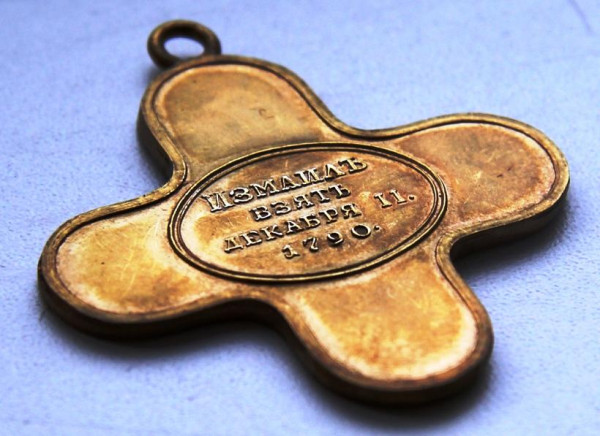
\includegraphics[width=0.9\textwidth]{images/medal-1.jpg}
		\end{column}
		\begin{column}{0.45\textwidth}

			Крест был сделан из золота. Размер креста — 46 × 46 мм. Крест равносторонний четырёхконечный с закруглёнными окончаниями. С двух сторон нанесены надписи.

		\end{column}
	\end{columns}
\end{frame}
\begin{frame}{}
	\begin{columns}
		\begin{column}{0.45\textwidth}

			Крест имел ушко для крепления к ленте. Носили его на груди на Георгиевской ленте.

		\end{column}
		\begin{column}{0.45\textwidth}

			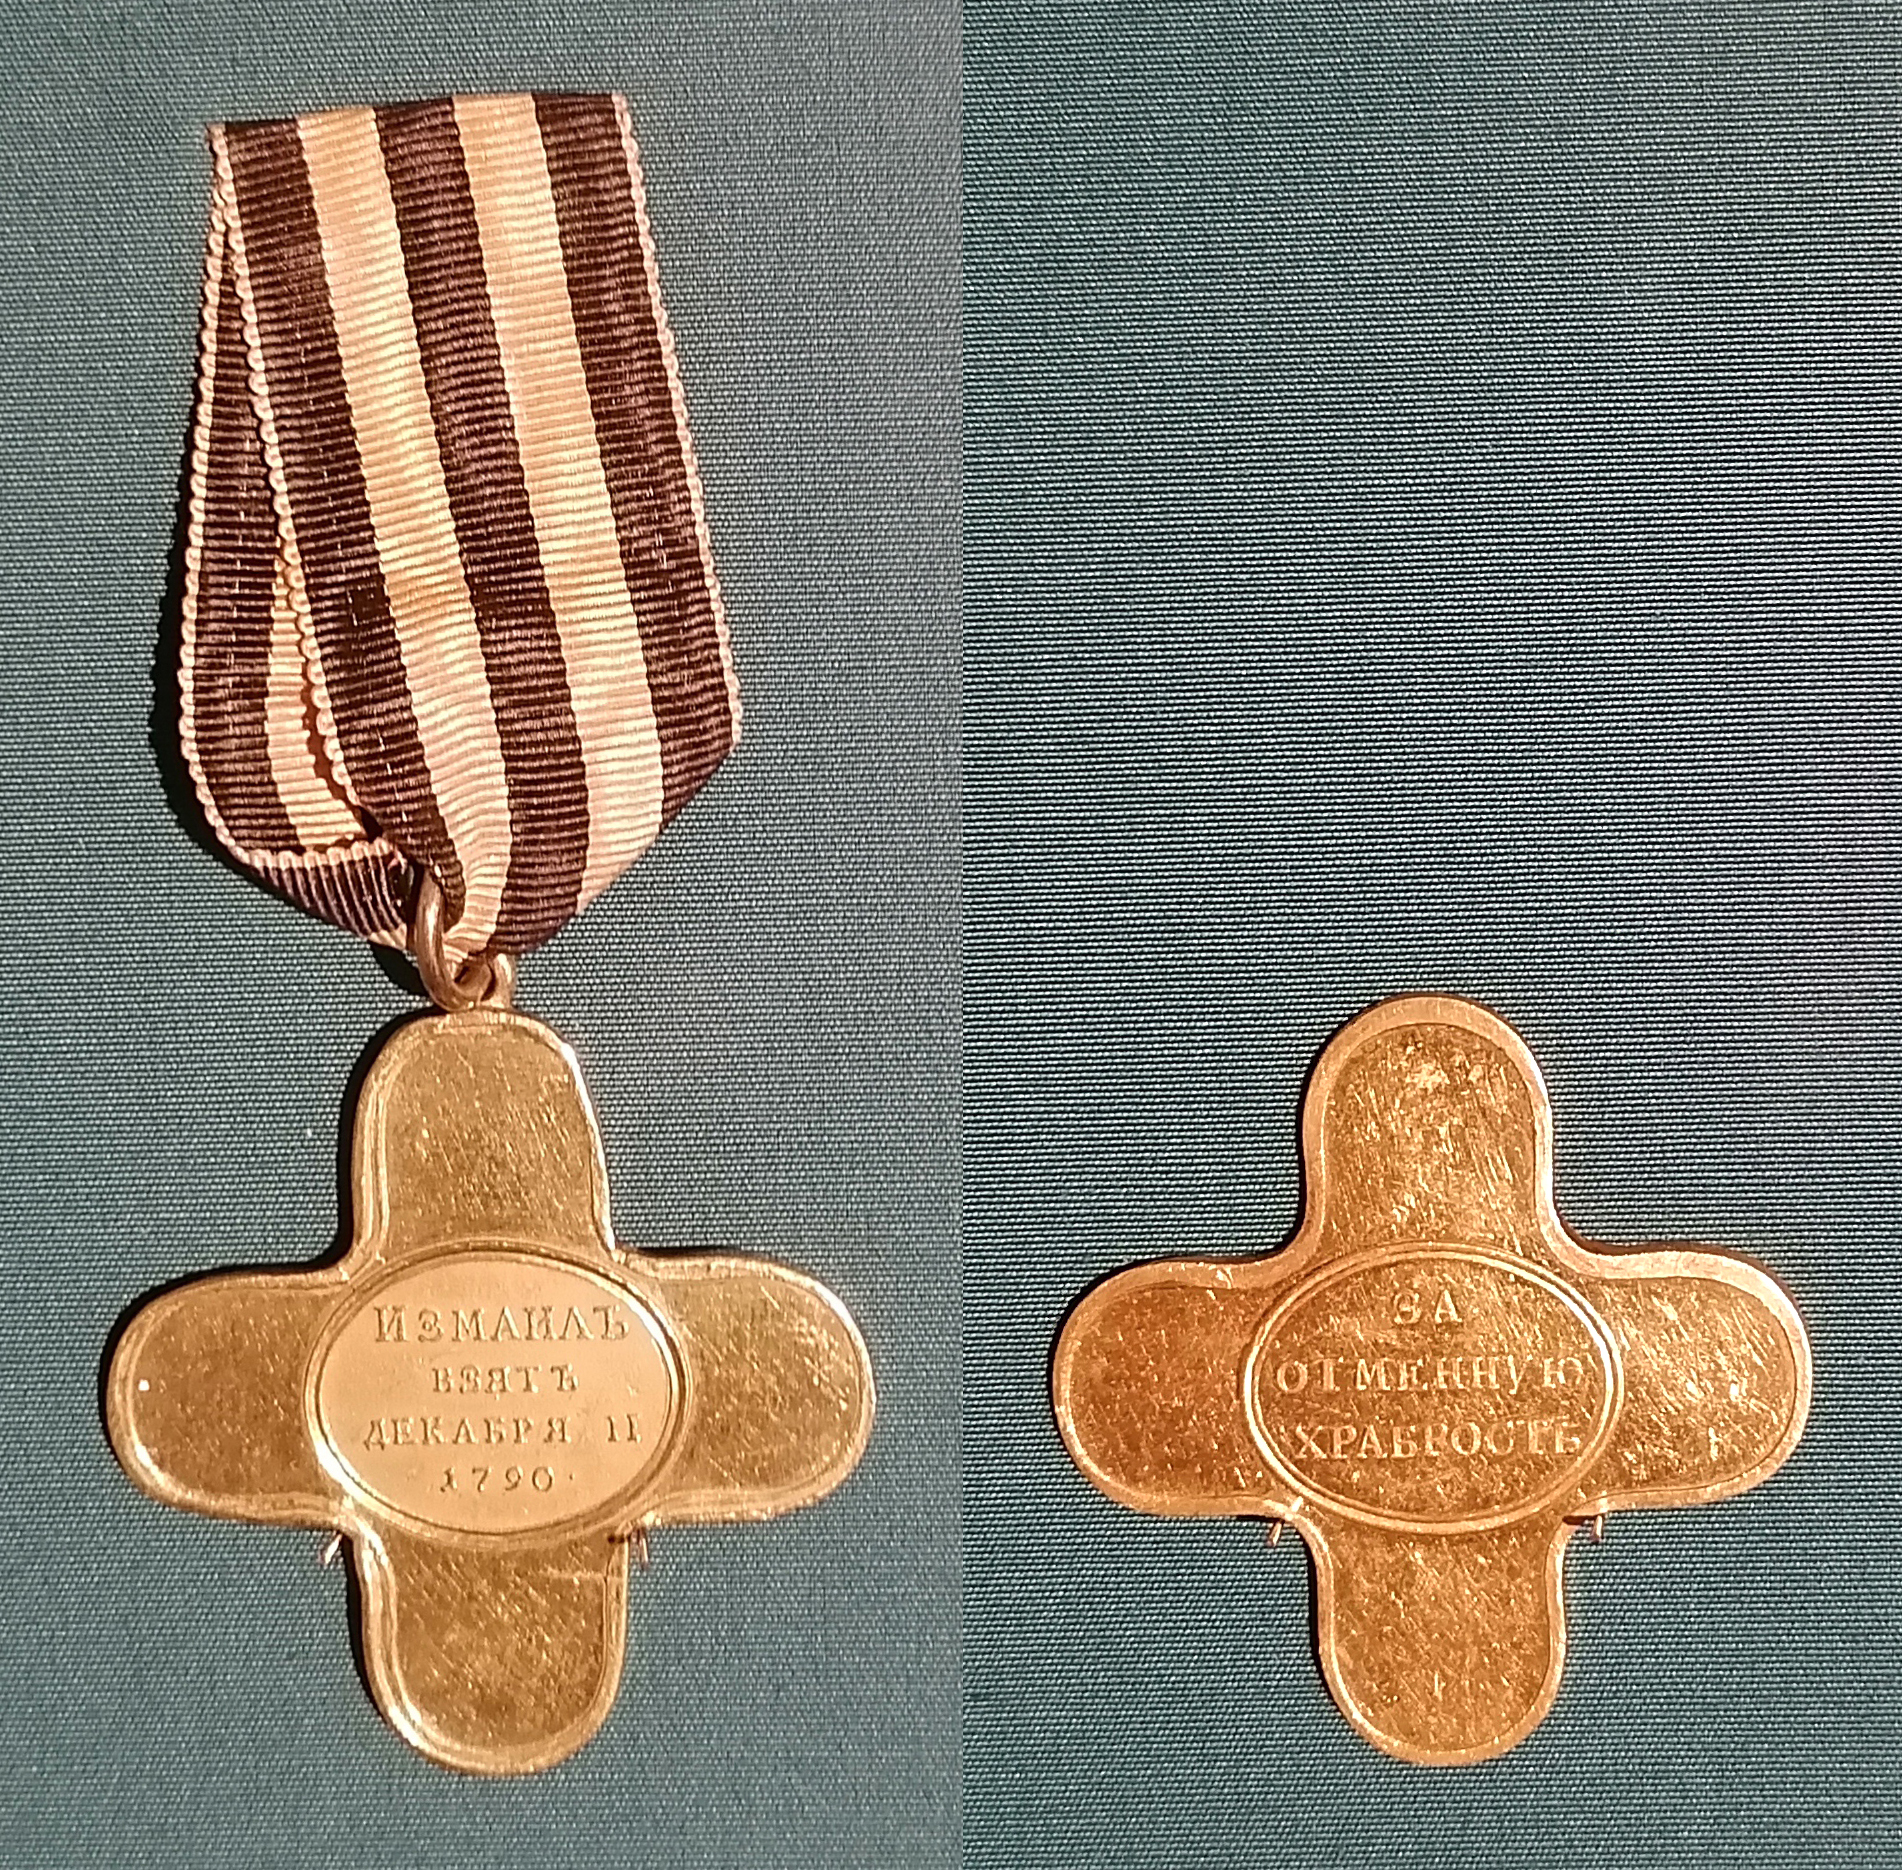
\includegraphics[width=0.9\textwidth]{images/medal-2.jpg}

		\end{column}
	\end{columns}
\end{frame}
\begin{frame}{}
	\begin{columns}
		\begin{column}{0.45\textwidth}
			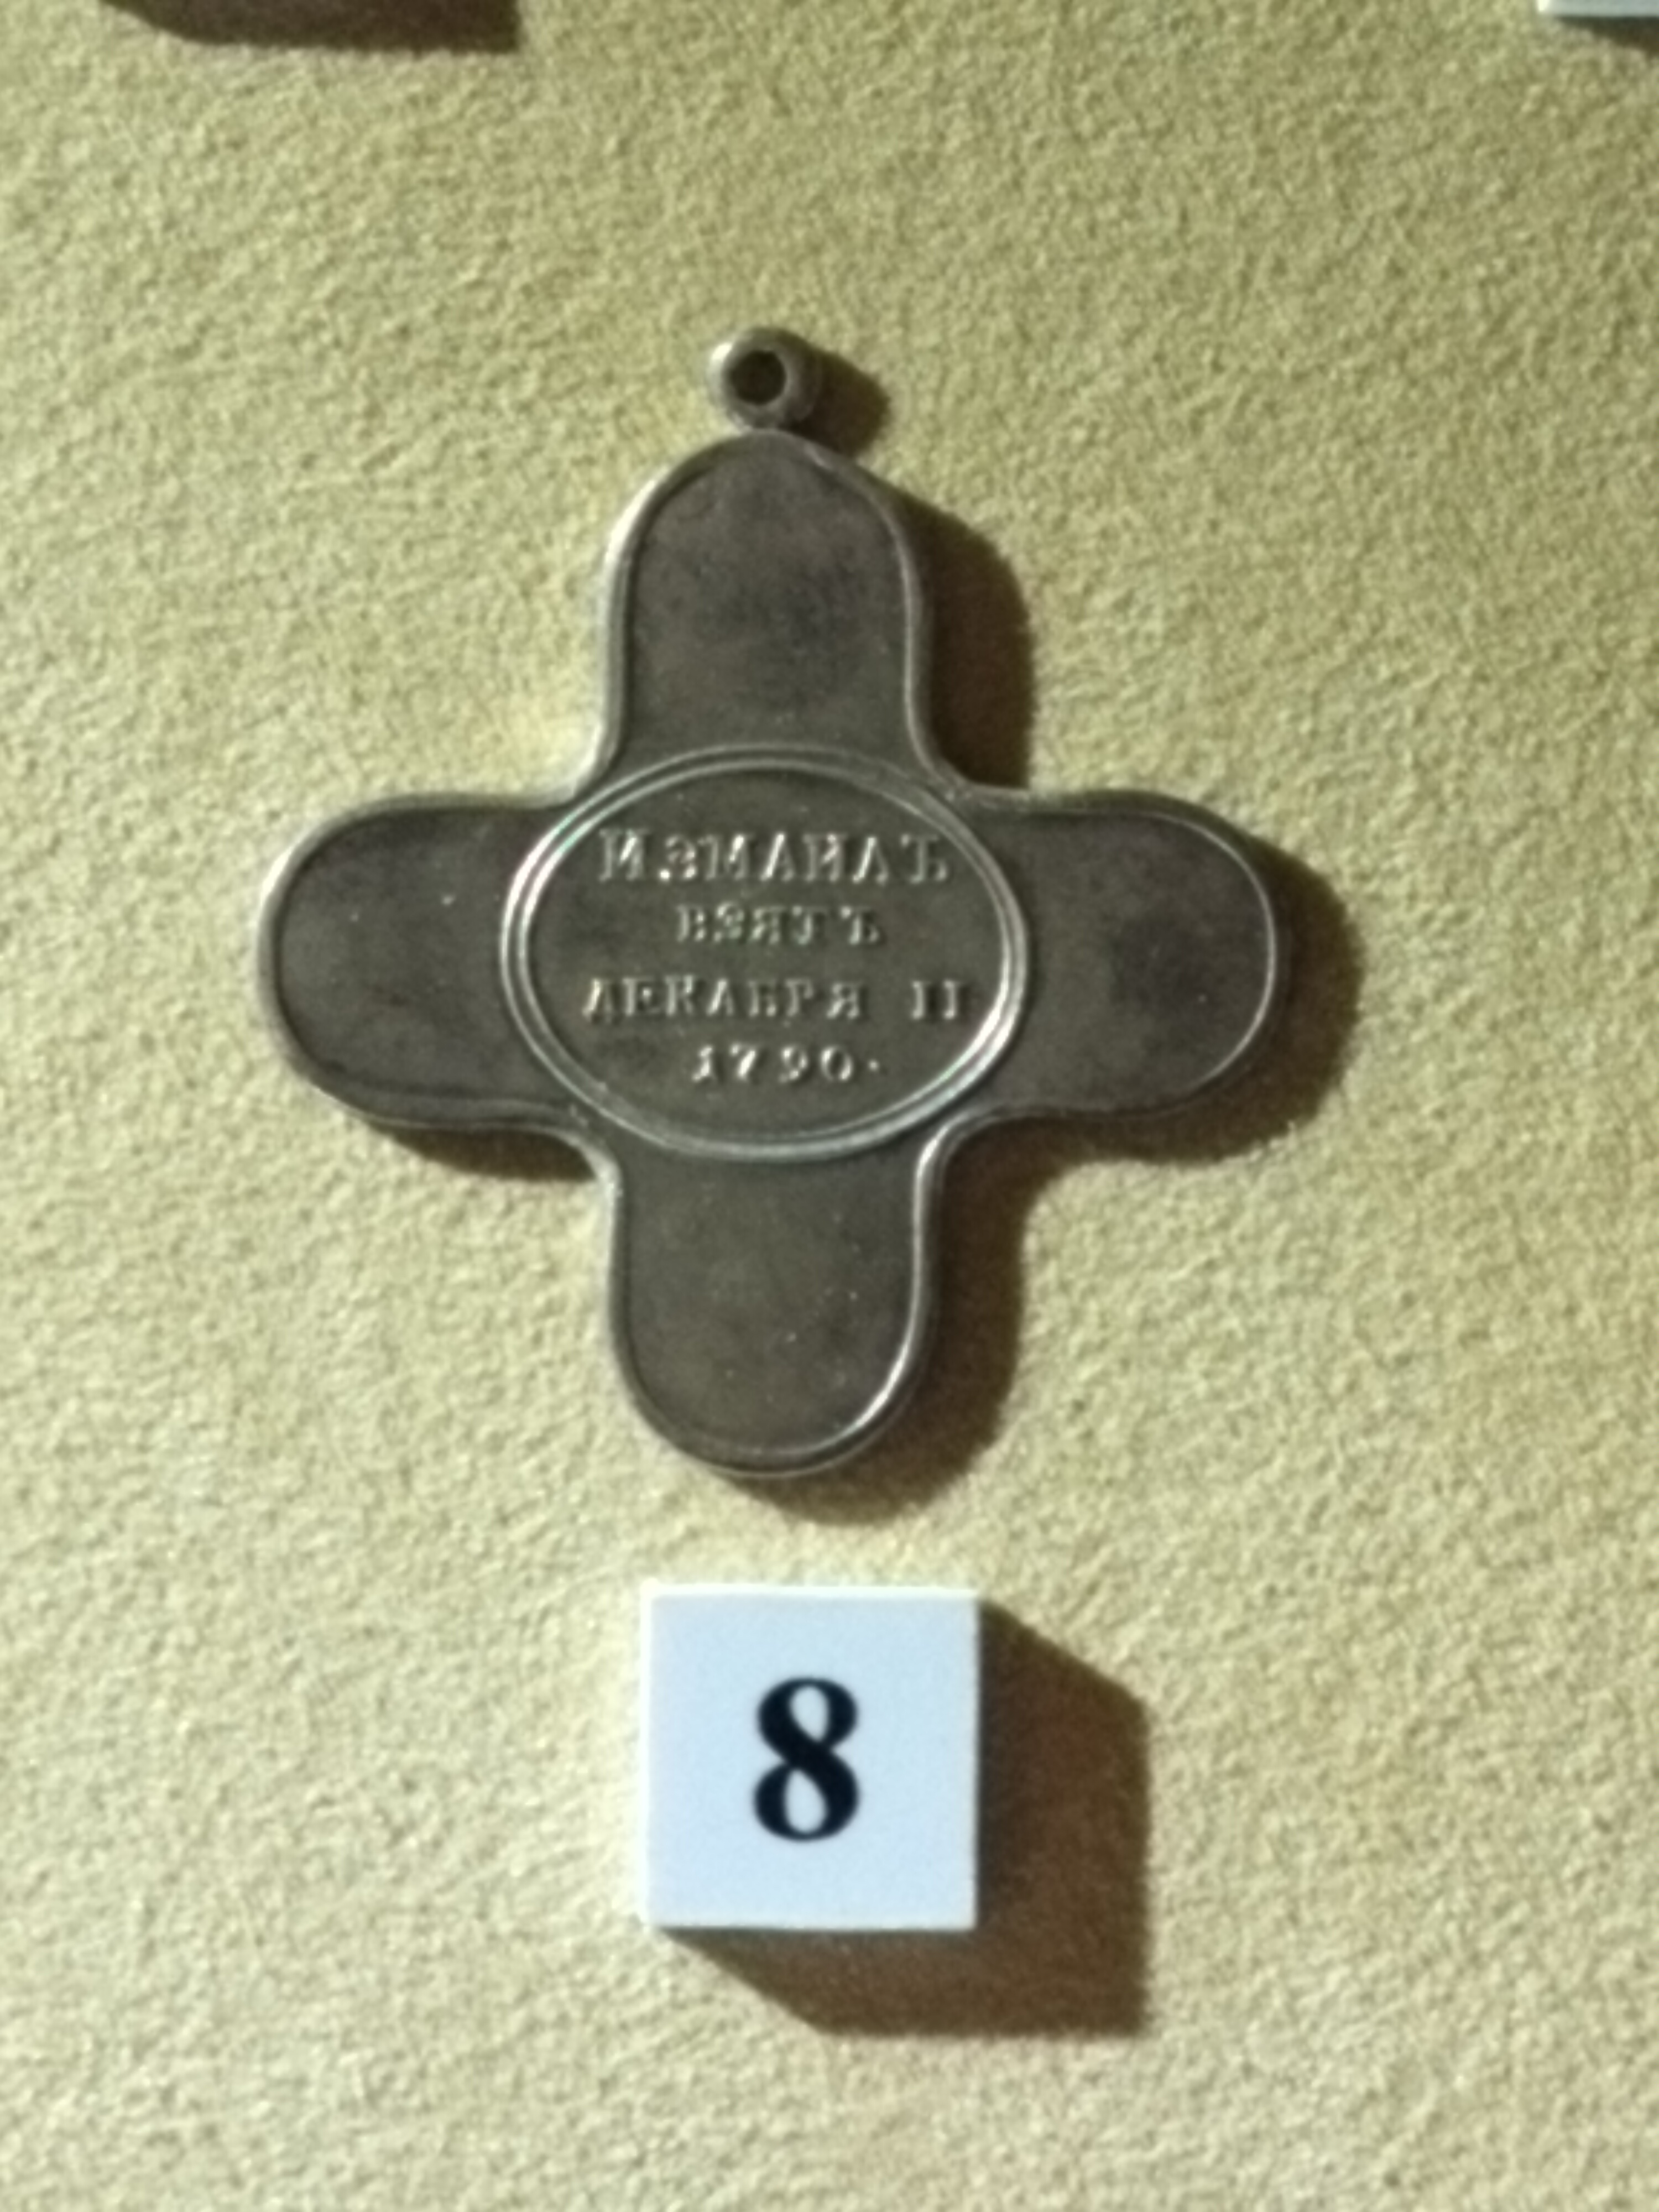
\includegraphics[width=0.9\textwidth]{images/medal-3.jpg}
		\end{column}
		\begin{column}{0.45\textwidth}

			Надпись на лицевой стороне:

			\textbf{«ЗА ОТМЕННУЮ ХРАБРОСТЬ»}.

			С обратной стороны:

			\textbf{«ИЗМАИЛЪ ВЗЯТЪ ДЕКАБРЯ 11 1790·»}.

		\end{column}
	\end{columns}
\end{frame}

\section{References}

\begin{frame}[t]{References}
	\printbibliography
	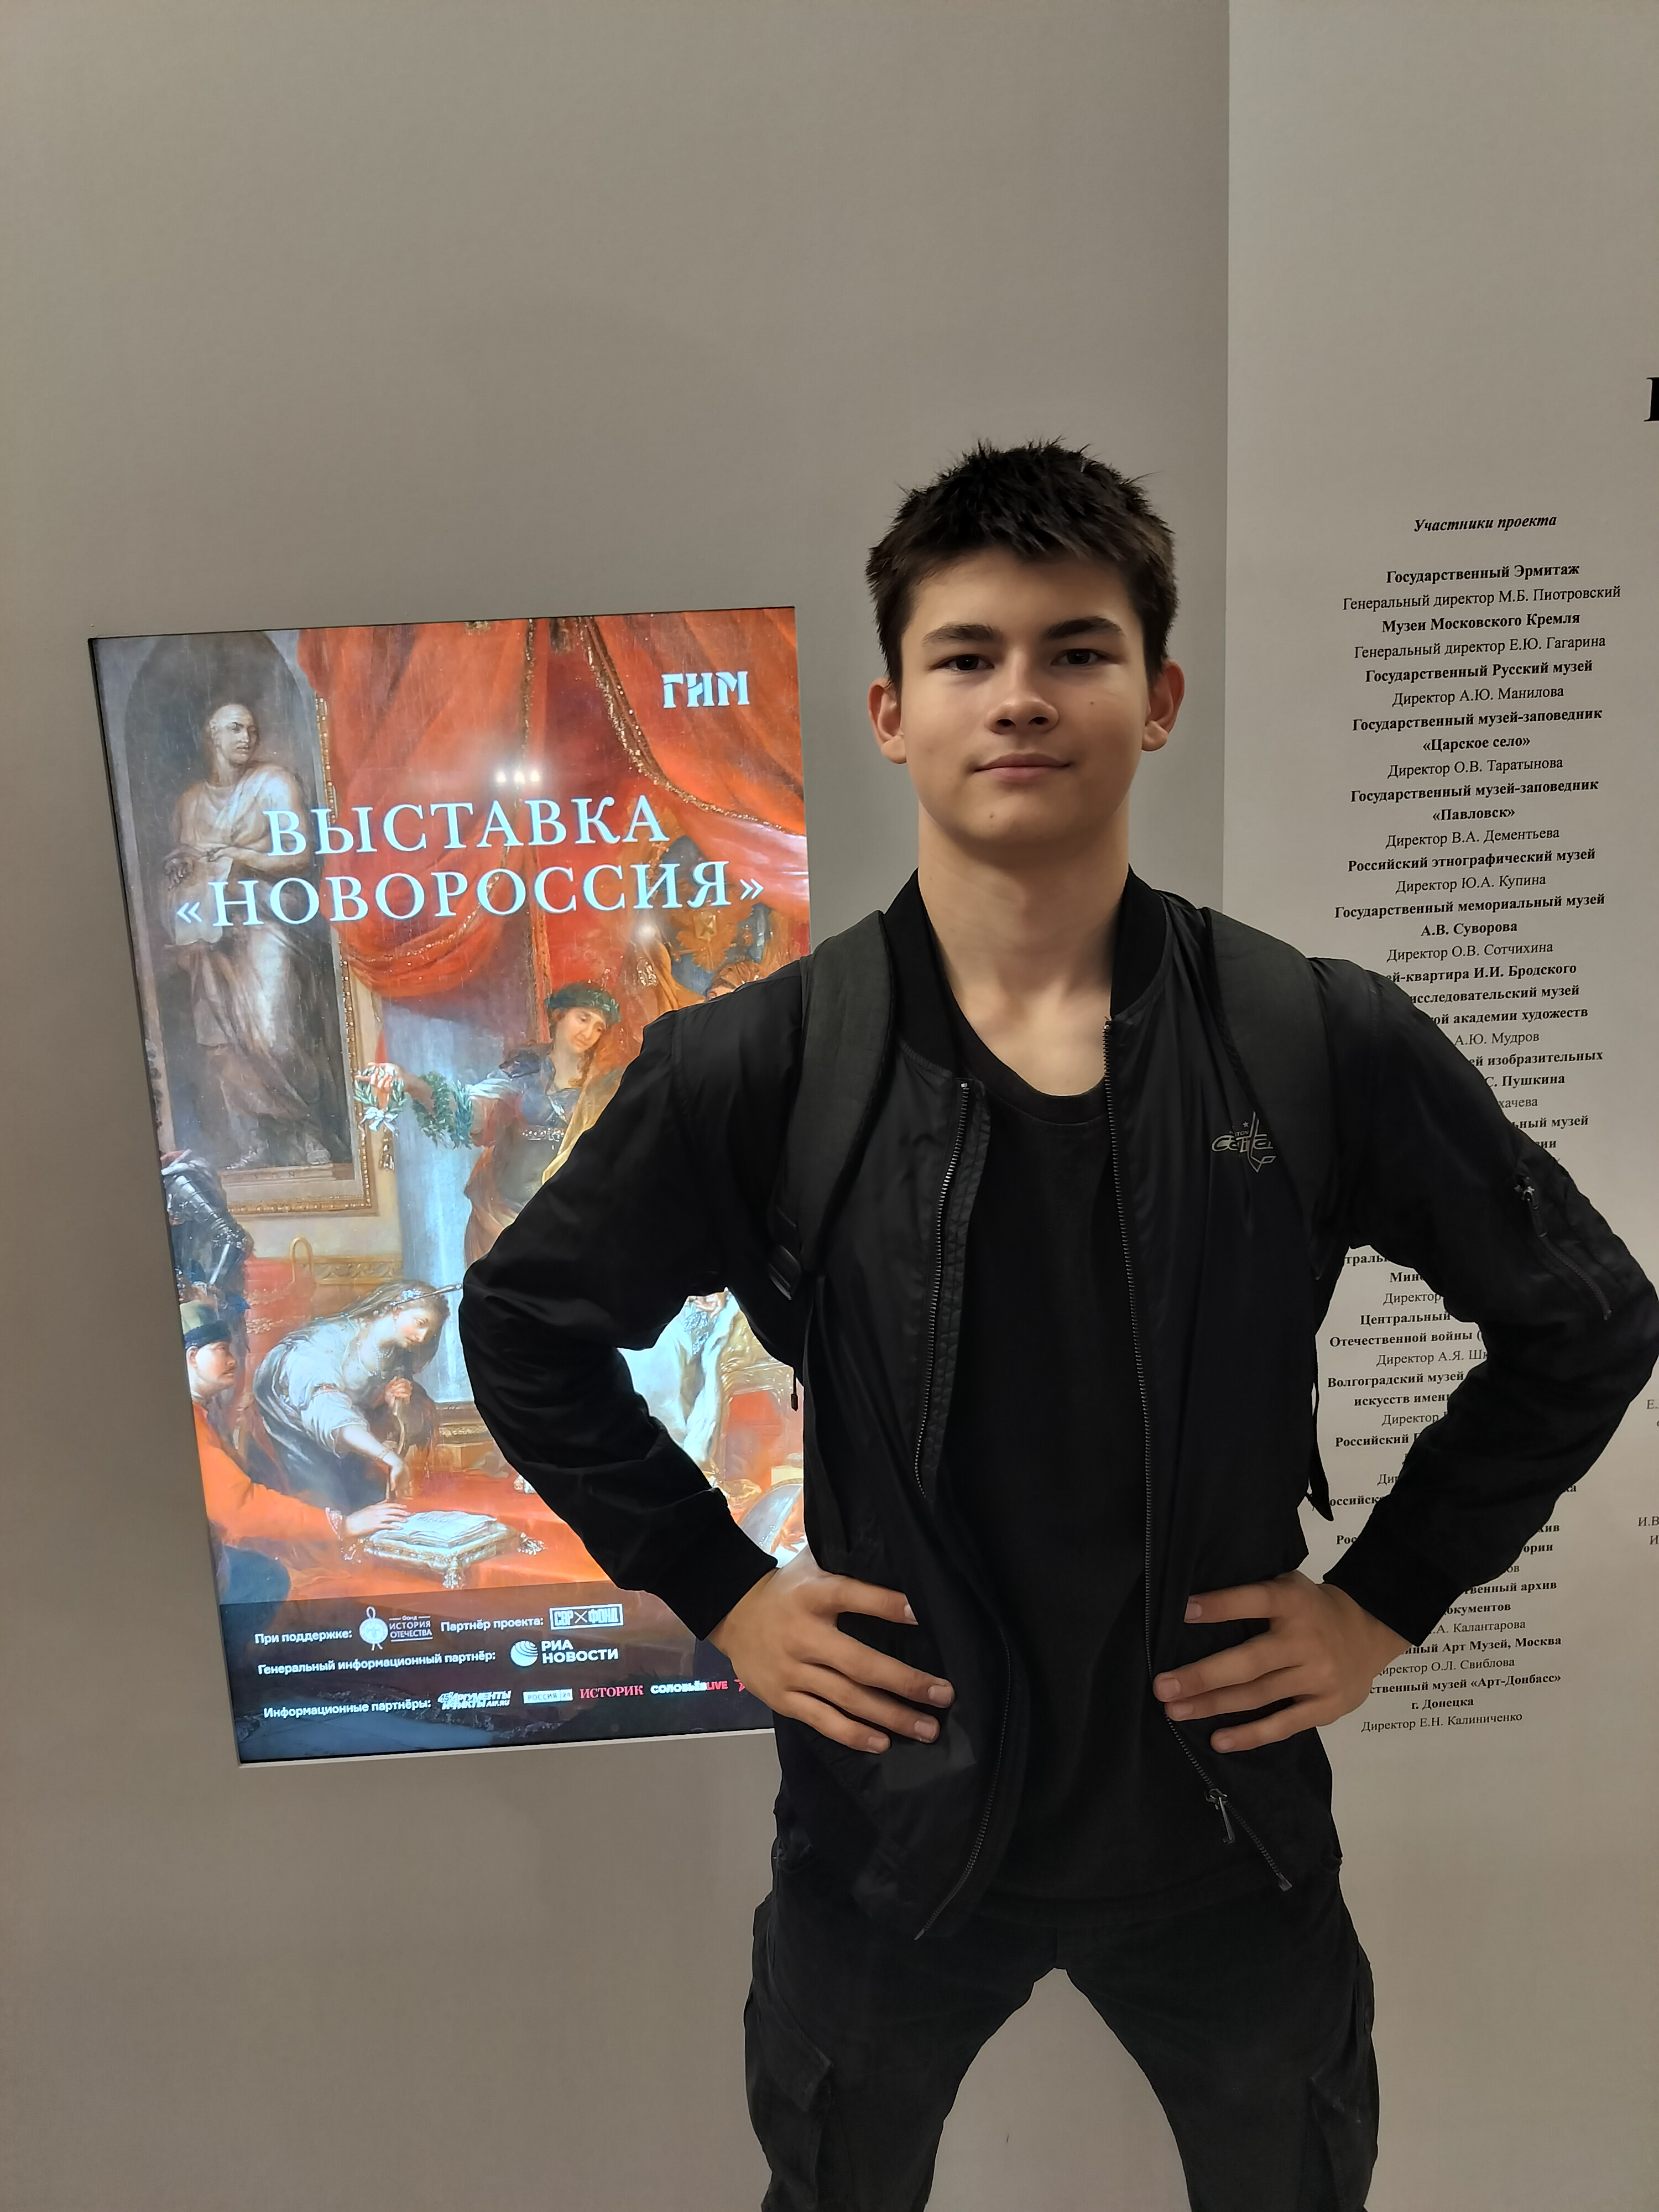
\includegraphics[width=0.4\textwidth]{images/self.jpg}
	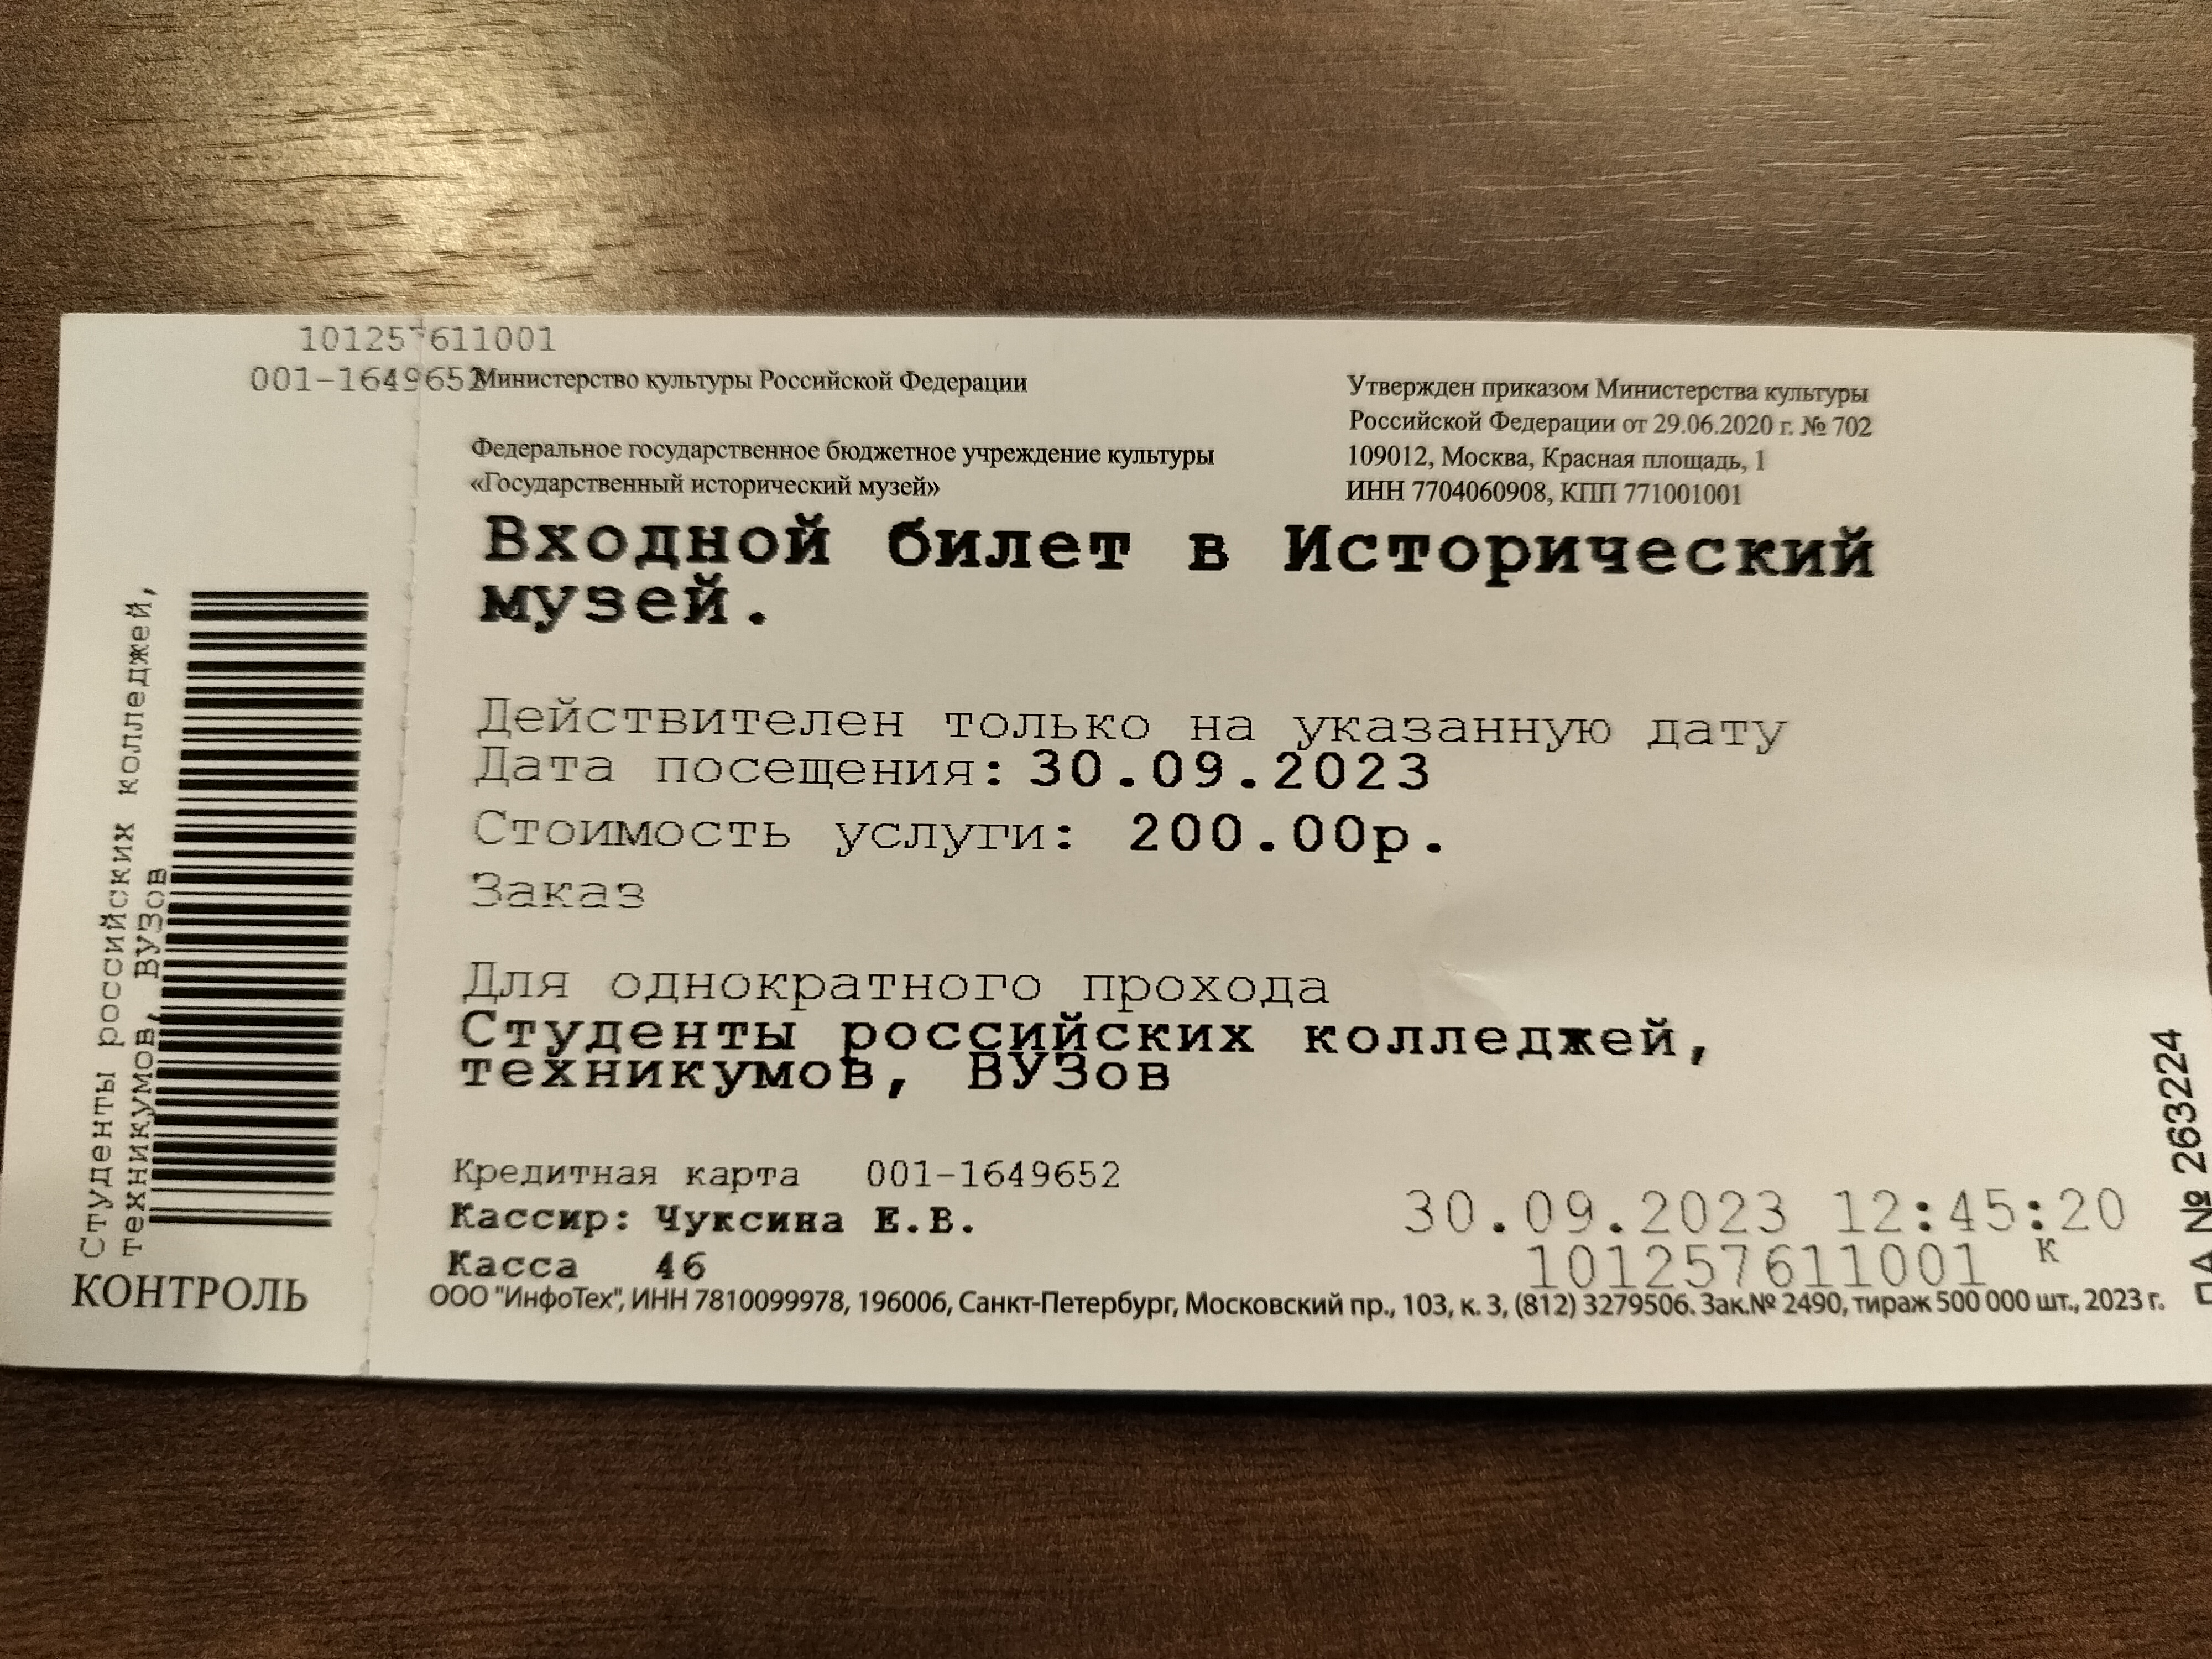
\includegraphics[width=0.4\textwidth]{images/ticket.jpg}
	\url{}
	\url{}
\end{frame}

\section{Благоданость}
\begin{frame}
	\centering
	\huge
	Спасибо за внимание!
\end{frame}


\end{document}
